\documentclass[12pt]{article}

% UTF-8 encoding
\usepackage[utf8]{inputenc}
\usepackage[T1]{fontenc}

% Page setup
\usepackage[margin=1in]{geometry}
\usepackage{setspace}
\onehalfspacing

% Math and symbols
\usepackage{amsmath,amssymb}

% Graphics
\usepackage{graphicx}
\usepackage{float}
\usepackage{pgfplots}
\pgfplotsset{compat=1.17}

% Tables
\usepackage{booktabs}
\usepackage{array}
\usepackage{multirow}
\usepackage{threeparttable}

% Bibliography
\usepackage{natbib}
\bibliographystyle{aer}

% Hyperlinks
\usepackage{hyperref}
\hypersetup{
    colorlinks=true,
    linkcolor=blue,
    citecolor=blue,
    urlcolor=blue
}

% Captions
\usepackage{caption}
\captionsetup{font=small,labelfont=bf}

% Section formatting
\usepackage{titlesec}
\titleformat{\section}{\large\bfseries}{\thesection.}{0.5em}{}
\titleformat{\subsection}{\normalsize\bfseries}{\thesubsection}{0.5em}{}

% Custom commands
\newcommand{\E}{\mathbb{E}}

\title{The Labor Supply Effects of Texas's Nurse Mandatory Overtime Ban: A Difference-in-Differences Analysis}
\author{APEP Autonomous Research\thanks{%
  Autonomous Policy Evaluation Project.
  This paper was autonomously generated using Claude Code.
  Repository: https://github.com/dakoyana/auto-policy-evals nd @dakoyana}}
\date{January 2026}

\begin{document}

\maketitle

\begin{abstract}
\noindent
We examine the labor supply effects of Texas's 2009 nurse mandatory overtime ban using a difference-in-differences design comparing Texas nurses to nurses in control states (Arizona, Florida, Georgia, Louisiana, Oklahoma) that lacked similar regulations. Using American Community Survey PUMS data from 2007--2012 covering 37,801 nurse observations, we find no statistically significant effect on average weekly hours worked (DiD estimate: +0.08 hours, SE: 0.29). Both Texas and control states experienced similar declines in average hours over the study period (approximately 0.9--1.0 hours), consistent with parallel trends in the absence of differential policy effects. We find suggestive evidence of positive employment effects (+1.1 percentage points), consistent with hospitals hiring additional nurses to compensate for reduced overtime capacity. Heterogeneity analysis reveals larger (but statistically insignificant) positive effects among male nurses (+1.35 hours). Our null result on hours suggests either that mandatory overtime was not widespread before the ban, that hospitals substituted toward voluntary overtime, or that household surveys cannot distinguish between mandatory and voluntary overtime. These findings contribute to the literature on occupational regulation and healthcare workforce policy, informing ongoing debates about nurse working conditions and patient safety.
\end{abstract}

\vspace{1em}
\noindent\textbf{JEL Codes:} J22, J32, I18, J44 \\
\noindent\textbf{Keywords:} nurse labor supply, mandatory overtime, occupational regulation, difference-in-differences, healthcare workforce

\newpage

\section{Introduction}

Nurse staffing and working conditions represent central concerns in healthcare policy debates across the United States. The nursing profession faces persistent workforce challenges, including chronic shortages, high turnover rates, and concerns about burnout and job satisfaction \citep{aiken2002hospital, buerhaus2009future}. Extended work hours and mandatory overtime have been identified as contributing factors to nurse fatigue, with potential consequences for both worker well-being and patient safety \citep{rogers2004work, trinkoff2011overtime}. In response to these concerns, numerous states have enacted legislation restricting the use of mandatory overtime for nurses, with Texas implementing such a ban effective September 1, 2009.

This paper examines whether Texas's nurse mandatory overtime ban affected nurse labor supply, as measured by weekly hours worked and employment. We employ a difference-in-differences (DiD) design comparing nurses in Texas to nurses in control states---Arizona, Florida, Georgia, Louisiana, and Oklahoma---that did not have similar restrictions during our study period of 2007 through 2012. This design allows us to difference out common trends affecting all states while isolating the effect of the Texas-specific policy change.

Economic theory yields ambiguous predictions about the effects of mandatory overtime bans on nurse labor supply. Standard labor supply models suggest that if mandatory overtime was common before the ban, restricting it should reduce average hours worked among nurses by eliminating the ability of employers to require additional work beyond scheduled shifts. However, labor demand considerations introduce countervailing forces: hospitals may respond to overtime restrictions by hiring additional nurses to maintain adequate staffing levels, offering premium pay for voluntary overtime, or adjusting scheduling practices in ways that partially offset the direct effects of the regulation. The net effect on observed hours thus depends on the prevalence of mandatory overtime pre-ban, the elasticity of nurse labor supply to voluntary overtime opportunities, and hospital demand responses.

Using American Community Survey (ACS) Public Use Microdata Sample (PUMS) data, we find a null effect on average weekly hours worked. Our DiD estimate is +0.08 hours (approximately 5 minutes per week), which is not statistically significant with a t-statistic of 0.27. Both Texas and control states experienced similar declines in average hours over the study period---Texas nurses worked approximately 0.91 fewer hours per week in the post-period, while control state nurses worked 0.99 fewer hours per week. This parallel decline is consistent with common trends affecting all states and supports the identifying assumption of our research design.

We find suggestive evidence of positive employment effects, with a DiD estimate of +1.07 percentage points. This pattern is consistent with theoretical predictions that hospitals would hire additional nurses to compensate for reduced overtime capacity. However, this estimate is imprecisely estimated and should be interpreted with caution.

Several interpretations of our null result on hours are possible. First, mandatory overtime may not have been widespread in Texas hospitals before the 2009 ban, limiting the scope for the policy to affect observed hours. Second, the ban restricted mandatory overtime but not voluntary overtime, so hospitals may have shifted from requiring overtime to offering premium pay for voluntary additional work. The ACS measures usual hours worked but cannot distinguish between mandatory and voluntary overtime, potentially masking compositional changes in how overtime occurs. Third, hospitals may have made scheduling adjustments that maintained similar average hours while eliminating mandatory overtime specifically.

This paper contributes to three strands of literature. First, we contribute to the economics of healthcare workforce policy by providing quasi-experimental evidence on nurse overtime regulations. While prior research has examined nurse overtime in cross-sectional or multi-state panel contexts \citep{bae2014assessing, ahn2023mandatory}, our study provides individual-level estimates using a well-defined policy change with pre-registered analysis. Second, we contribute to the literature on occupational regulation more broadly, examining how restrictions on working conditions affect labor supply \citep{kleiner2006licensing, thornton2018role}. Third, we provide evidence relevant to ongoing policy debates about nurse working conditions and patient safety, topics of continued legislative interest across states.

The remainder of this paper proceeds as follows. Section 2 reviews the related literature on nurse labor supply, overtime regulation, and healthcare workforce policy. Section 3 describes the institutional background of nurse overtime regulations and the Texas policy specifically. Section 4 presents our data sources and sample construction. Section 5 details our empirical strategy and identification assumptions. Section 6 presents results, and Section 7 discusses interpretation and implications. Section 8 concludes.

\section{Literature Review}

\subsection{Nurse Labor Supply and Working Conditions}

The economics of nurse labor supply has generated substantial research attention, motivated by persistent concerns about nursing shortages and their implications for healthcare delivery. Foundational work by \cite{shields2004labor} provides a comprehensive survey of the nurse labor market, documenting the unique features of this occupation including high female labor force participation rates, substantial variation in hours worked, and sensitivity to wage and non-wage job characteristics.

Research on the determinants of nurse labor supply has emphasized the importance of working conditions alongside wages. \cite{aiken2002hospital} documented significant associations between nurse staffing levels, working conditions, and both nurse job satisfaction and patient outcomes. Hospitals with higher nurse-to-patient ratios exhibited lower rates of nurse burnout and job dissatisfaction, suggesting that working conditions play an important role in nurse labor supply decisions. \cite{mcgillis2005nursing} extended this work by examining the relationship between nurse staffing decisions and organizational characteristics, finding that hospitals adjust staffing levels in response to patient acuity and financial pressures.

The role of overtime in nurse labor supply has received particular attention due to its implications for both worker welfare and patient safety. \cite{rogers2004work} documented that hospital staff nurses frequently work beyond scheduled hours, with the majority of extended shifts unplanned. Their analysis found that the risk of making an error increased significantly when nurses worked longer than 12.5 hours or worked overtime. \cite{trinkoff2011overtime} provided complementary evidence linking nurse work schedule characteristics to patient mortality, finding that schedules with long hours, lack of days off, and overtime work were associated with worse patient outcomes.

\subsection{Mandatory Overtime Regulation}

Policy responses to concerns about nurse overtime have taken various forms across states. \cite{bae2014assessing} provided a comprehensive assessment of state nurse work hour regulations, documenting the substantial variation in policy approaches. Some states enacted outright bans on mandatory overtime, while others implemented restrictions with exceptions for emergencies or established maximum consecutive work hours. Their analysis found that state regulations reduced the odds of nurses working overtime, though effects varied by the stringency of the regulation.

The theoretical predictions of overtime regulation effects are ambiguous. On one hand, restrictions on mandatory overtime should directly reduce overtime hours among nurses who would otherwise be required to work additional shifts. On the other hand, hospitals face strong incentives to maintain adequate staffing levels to ensure patient safety and meet regulatory requirements. \cite{dall2014nursing} documented the substantial costs of nurse turnover and the value hospitals place on maintaining stable nursing workforces, suggesting that hospitals may respond to overtime restrictions by adjusting hiring, scheduling, or compensation practices.

Recent work by \cite{ahn2023mandatory} examined the effects of mandatory overtime bans on nurse labor supply using administrative data from a single hospital system. Their analysis found modest effects on overtime hours, with larger impacts among nurses with stronger preferences for shorter workweeks. This within-hospital analysis provides valuable micro-level evidence but may not generalize to broader labor market effects captured by population surveys.

\subsection{Economic Effects of Occupational Regulation}

Our paper also relates to the broader literature on occupational regulation and its labor market effects. \cite{kleiner2006licensing} provided foundational analysis of occupational licensing, documenting substantial growth in the share of workers requiring licenses and examining the wage and employment effects of licensing requirements. Their work highlighted the dual nature of occupational regulation: restrictions can protect consumers by ensuring quality but may also reduce competition and raise prices.

\cite{thornton2018role} examined the effects of specific occupational regulations on labor supply, finding that regulations can affect both the extensive margin (labor force participation) and intensive margin (hours worked). Their framework suggests that regulations restricting working conditions may have offsetting effects: reducing hours among those who would prefer to work more while potentially attracting workers who prefer shorter workweeks or less demanding conditions.

The healthcare context introduces additional considerations. \cite{propper2006impacts} examined how labor market conditions affect the behavior of public sector healthcare workers, finding that outside options significantly influenced effort and retention. This suggests that nurse responses to overtime regulation may depend on labor market conditions and alternative employment opportunities.

\subsection{Identification Challenges}

Identifying causal effects of overtime regulations presents methodological challenges. State-level policy variation may be correlated with unobserved factors affecting nurse labor supply, and different states may adopt policies at different times for different reasons. Recent advances in difference-in-differences methodology have highlighted these concerns for settings with staggered treatment adoption \citep{goodmanbacon2021, callaway2021}. However, our setting involves a single treatment event (Texas's 2009 policy), avoiding the negative weighting problems that can arise with multiple treatment cohorts.

Prior studies have addressed identification through various approaches. \cite{bae2014assessing} used state-year panel data with state fixed effects, effectively comparing within-state changes over time. \cite{ahn2023mandatory} used administrative data from a single hospital system, leveraging within-hospital variation. Our approach uses individual-level survey data to compare nurses in Texas to nurses in control states without overtime restrictions, differencing out common trends while providing population-representative estimates.

\section{Institutional Background}

\subsection{Nurse Overtime in the United States}

Nursing in the United States has historically involved substantial work hours, with the American Hospital Association documenting that the average nurse work year exceeds the national average by approximately 200 hours \citep{aha2012}. This pattern reflects the around-the-clock nature of hospital operations, the challenges of matching staffing to fluctuating patient census, and the specialized skills that make nurse labor difficult to substitute on short notice.

Mandatory overtime---the requirement that nurses work beyond their scheduled shifts---emerged as a common practice in many hospitals, particularly during periods of high patient volume or staff shortages. Unlike voluntary overtime, which nurses may decline without consequence, mandatory overtime can be a condition of continued employment. Hospitals facing staffing shortages often viewed mandatory overtime as a necessary tool for maintaining adequate patient care coverage, particularly in specialized units where specific skills are required.

The practice of mandatory overtime attracted criticism from nursing organizations and patient safety advocates throughout the 1990s and 2000s. The American Nurses Association adopted policy positions opposing mandatory overtime, citing concerns about nurse fatigue, stress, and the potential for errors. The Institute of Medicine's influential 2004 report, ``Keeping Patients Safe: Transforming the Work Environment of Nurses,'' recommended that healthcare organizations ``implement policies and practices that prevent nurses from providing patient care when fatigued'' and specifically suggested limits on work hours \citep{iom2004}.

Research findings supported these concerns. Studies documented associations between extended work hours and adverse outcomes including medication errors, needle stick injuries, and patient falls. The biological and psychological effects of fatigue were well-established, and the high-stakes nature of nursing work---where errors can have serious consequences---heightened concerns about overtime-induced fatigue.

\subsection{State Policy Responses}

Beginning in the early 2000s, states began enacting legislation restricting mandatory overtime for nurses. These policies took various forms depending on state legislative processes and healthcare industry involvement. Some states enacted outright bans on mandatory overtime except in declared emergencies. Others established maximum consecutive work hours or required minimum rest periods between shifts. Still others implemented disclosure requirements or established committees to review overtime practices.

By 2012, approximately 18 states had enacted some form of nurse overtime restriction, though the specific provisions varied substantially \citep{bae2014assessing}. California, often a leader in labor regulation, enacted comprehensive nurse staffing ratios in 2004, which indirectly affected overtime practices by requiring minimum nurse-to-patient ratios. Other states focused specifically on overtime restrictions without broader staffing requirements.

The variation in state policies reflects different approaches to balancing worker protection with healthcare operational flexibility. Strict bans provide clear protection for nurses but may create challenges for hospitals during genuine emergencies or unexpected staffing shortages. More flexible approaches allow for emergency exceptions but may be more difficult to enforce and may leave nurses feeling pressure to accept ``voluntary'' overtime.

\subsection{Texas Senate Bill 476}

On September 1, 2009, Texas implemented Health and Safety Code Chapter 258, which was enacted via Senate Bill 476 by the 81st Legislature. The legislation represented a significant change in how Texas hospitals could manage nurse staffing.

The law prohibits hospitals from requiring nurses---specifically, registered nurses (RNs) and licensed vocational nurses (LVNs)---to work mandatory overtime. Mandatory overtime is defined broadly as work beyond scheduled hours or days, regardless of the length of scheduled shifts or the number of scheduled shifts per week. This definition captured the common practice of extending shifts beyond scheduled end times.

The law included important protections for nurses who decline overtime. Hospitals are prohibited from suspending, terminating, or otherwise disciplining nurses who refuse mandatory overtime. This anti-retaliation provision was designed to ensure that the overtime restriction had practical effect, preventing hospitals from pressuring nurses to accept ``voluntary'' overtime through implicit threats.

The law carved out exceptions for genuine emergencies. Hospitals may require overtime when a state of disaster has been declared by the governor or president, or in emergency situations as defined by hospital administrators. These exceptions recognized that certain circumstances---natural disasters, mass casualty events, or other emergencies---may require extraordinary staffing measures.

Implementation of the law involved notification requirements and enforcement mechanisms. The Texas Board of Nursing received authority to investigate complaints regarding mandatory overtime violations, and hospitals found in violation could face administrative penalties.

\subsection{Control States}

Our analysis uses nurses in Arizona, Florida, Georgia, Louisiana, and Oklahoma as controls. These states were selected because they did not have mandatory overtime restrictions for nurses during our study period and represent the Sun Belt region geographically proximate to Texas.

Arizona had not enacted nurse overtime legislation during our study period. The state's healthcare sector, centered around Phoenix and Tucson, operated under standard federal labor law provisions without additional state restrictions on overtime practices.

Florida, with its large healthcare sector serving both resident and visitor populations, similarly lacked mandatory overtime restrictions. The state's right-to-work laws and generally business-friendly regulatory environment extended to healthcare staffing practices.

Georgia's healthcare sector, anchored by major systems in Atlanta, operated without state-level overtime restrictions. Louisiana and Oklahoma, with smaller healthcare sectors, similarly relied on federal labor law without additional state restrictions on nurse overtime.

These states provide a reasonable comparison group for Texas. They share regional characteristics including climate, demographic patterns, and economic structure. Their healthcare sectors face similar challenges in nurse recruitment and retention. The absence of overtime restrictions in these states during our study period allows us to observe what happened to nurse hours in the absence of policy intervention.

\section{Data}

\subsection{Data Source}

We use the American Community Survey (ACS) Public Use Microdata Sample (PUMS) 1-year data files for 2007, 2008, 2010, 2011, and 2012. The ACS is a continuous survey conducted by the U.S. Census Bureau, providing annual data on demographic, social, economic, and housing characteristics of the U.S. population. The PUMS files contain individual-level records with detailed information about each respondent, enabling analysis of specific population subgroups.

We exclude 2009 from our analysis because the policy took effect on September 1, 2009, making that year a transition period. ACS interviews are conducted throughout the calendar year, so 2009 responses would reflect a mixture of pre-policy and post-policy labor market conditions. Excluding this year provides cleaner identification of pre-period and post-period effects.

The ACS provides several advantages for our analysis. First, its large sample size yields sufficient observations of nurses in both Texas and control states to enable precise estimation. Second, the survey includes key labor market variables including usual hours worked per week, employment status, and earnings. Third, the individual-level data allow us to control for demographic characteristics and examine heterogeneity across nurse subgroups.

The ACS also has limitations relevant to our analysis. Most importantly, the survey measures ``usual hours worked per week'' rather than actual overtime hours. Respondents are asked about their typical weekly hours, which may not precisely capture variation in mandatory versus voluntary overtime. The survey cannot distinguish between nurses required to work overtime and those who voluntarily accept additional shifts. This measurement limitation affects our ability to observe the mechanism through which the policy operates.

\subsection{Sample Construction}

Our sample includes individuals meeting several criteria designed to identify working-age nurses in the relevant states. We include individuals aged 21 through 64, capturing the primary working-age population while excluding very young workers who may still be in training and older workers who may be transitioning to retirement.

We identify nurses using ACS occupation codes. For the years 2007 through 2009, we use occupation code 3130 for registered nurses and 3500 for licensed practical nurses. For 2010 through 2012, following ACS coding changes, we use code 3255 for registered nurses and 3500 for licensed vocational/practical nurses. These codes correspond to the nursing occupations targeted by the Texas legislation.

We restrict the sample to individuals residing in Texas or one of the five control states: Arizona (state FIPS code 04), Florida (12), Georgia (13), Louisiana (22), or Oklahoma (40). This geographic restriction focuses our analysis on the comparison of interest while excluding states with their own overtime regulations that might confound the analysis.

We exclude self-employed nurses from the analysis. The mandatory overtime ban applied to hospitals, so nurses in independent practice or self-employed settings were not directly affected by the policy. Excluding self-employed nurses focuses the analysis on the population most likely to be treated by the policy. We identify self-employment using the class of worker variable (COW), excluding individuals coded as self-employed in an incorporated or unincorporated business.

\subsection{Variable Definitions}

Our primary outcome variable is usual weekly hours worked (WKHP). This variable captures the number of hours per week the respondent usually worked at their job during the past 12 months. For individuals with multiple jobs, it captures hours at the primary job. The variable ranges from 1 to 99 hours per week.

Our secondary outcome is employment status, constructed from the employment status recode variable (ESR). We code individuals as employed if they report being employed at work (ESR=1) or employed but not at work (ESR=2). We code other values (unemployed, not in labor force) as not employed.

Treatment status is determined by state of residence. Individuals residing in Texas (ST=48) are coded as treated, while individuals in control states are coded as controls.

The post-period indicator equals one for years 2010, 2011, and 2012, and zero for years 2007 and 2008.

We include demographic control variables in some specifications. Age (AGEP) captures years of age. Sex (SEX) equals 1 for male and 2 for female. Race (RAC1P) is included as categorical indicators. Education (SCHL) captures educational attainment.

All analyses use person weights (PWGTP) to ensure population representativeness. The ACS uses a complex survey design, and the person weights account for sampling probabilities and non-response adjustments.

\subsection{Sample Summary}

Our final sample includes 37,801 nurse observations across the six states and five years of data. Texas contributes 12,952 observations, while the control states contribute 24,849 observations. Florida is the largest control state with 11,367 observations, followed by Georgia (5,242), Arizona (3,052), Louisiana (2,972), and Oklahoma (2,216).

Sample sizes are reasonably balanced across years, ranging from 7,495 observations in 2010 to 7,660 observations in 2012. Within Texas, pre-period years (2007--2008) contribute 5,164 observations while post-period years (2010--2012) contribute 7,788 observations. The larger post-period sample reflects both the additional year of data and potential growth in the nursing workforce.

The demographic composition of our sample reflects the nursing profession. Approximately 90\% of sample observations are female, consistent with historical patterns of gender composition in nursing. The sample spans the full age range from 21 to 64, with substantial representation in middle-age categories where nurses have accumulated experience.

\section{Empirical Strategy}

\subsection{Identification}

We employ a classic difference-in-differences design to identify the effect of Texas's mandatory overtime ban on nurse labor supply. The fundamental identification challenge is that we cannot directly observe what would have happened to Texas nurses in the absence of the policy. Our strategy addresses this challenge by using nurses in control states as a counterfactual for the trajectory Texas nurses would have followed without the policy change.

The key identifying assumption is parallel trends: in the absence of the policy intervention, Texas and control state nurses would have experienced similar trends in outcomes. Under this assumption, any differential change in outcomes between Texas and control states after the policy can be attributed to the policy effect.

Our setting has an important feature that simplifies the econometric analysis. Unlike many state-level policy evaluations that involve staggered adoption---where different states adopt policies at different times---our setting involves a single treatment event. All Texas nurses were subject to the same policy change at the same time (September 1, 2009), and no control state nurses were treated during our study period.

This single-treatment feature means that traditional two-way fixed effects estimation does not suffer from the negative weighting problems documented in recent methodological work \citep{goodmanbacon2021, callaway2021}. Those problems arise when already-treated units serve as controls for newly-treated units, which can produce misleading estimates when treatment effects are heterogeneous. In our setting, there is only one treatment cohort, so this issue does not arise.

\subsection{Estimation}

Our primary specification estimates the following regression:

\begin{equation}
Y_{ist} = \alpha + \beta_1 \cdot \text{Texas}_s + \beta_2 \cdot \text{Post}_t + \tau \cdot (\text{Texas}_s \times \text{Post}_t) + X_{ist}'\gamma + \varepsilon_{ist}
\end{equation}

In this specification, $Y_{ist}$ denotes the outcome for nurse $i$ residing in state $s$ observed in year $t$. The indicator $\text{Texas}_s$ equals one for nurses residing in Texas and zero for nurses in control states. The indicator $\text{Post}_t$ equals one for years 2010 and later (post-policy) and zero for years 2007--2008 (pre-policy). The vector $X_{ist}$ includes demographic controls in some specifications.

The coefficient of primary interest is $\tau$, which captures the difference-in-differences estimate. This coefficient represents the differential change in outcomes for Texas nurses relative to control state nurses, comparing post-policy to pre-policy periods.

All regressions are weighted using person weights (PWGTP) to account for the complex survey design and ensure population representativeness of our estimates.

For statistical inference, we use heteroskedasticity-robust standard errors. Given the state-level policy variation, clustering at the state level would be conceptually appropriate but impractical given our small number of state clusters (6 states). We report robust standard errors and note that inference should be interpreted cautiously given the limited geographic variation.

\subsection{Identifying Assumptions}

The validity of our difference-in-differences design rests on several assumptions.

The parallel trends assumption requires that, in the absence of the policy, Texas and control state nurses would have experienced similar trends in outcomes. While this assumption cannot be directly tested, we assess its plausibility by examining pre-period trends. If Texas and control states exhibited similar trends before the policy---particularly if the differential between them was stable---this provides suggestive evidence supporting the parallel trends assumption.

The no anticipation assumption requires that nurses and hospitals did not substantially change behavior before September 2009 in anticipation of the policy. Given that the legislation was enacted during the 2009 legislative session, significant anticipation effects in 2007--2008 seem unlikely. However, anticipation effects in early 2009 are possible, which is why we exclude that year from the analysis.

The no spillovers assumption requires that the Texas policy did not affect nurse labor markets in control states. Spillovers could occur if, for example, Texas hospitals recruited nurses from control states to compensate for reduced overtime capacity, potentially increasing wages or hours in control states. While such spillovers are theoretically possible, the magnitude is likely small given the large nursing workforces in control states.

The stable composition assumption requires that the sample of nurses remained comparable across treatment and control groups over time. Violations could occur if the policy induced selective entry or exit from nursing in Texas. For example, if the overtime ban attracted nurses who prefer shorter workweeks, observed post-policy hours might reflect composition changes rather than behavioral responses among incumbent nurses.

\subsection{Event Study Specification}

To assess parallel trends and visualize the dynamic effects of the policy, we estimate an event study specification:

\begin{equation}
Y_{ist} = \alpha + \sum_{k \neq 2008} \gamma_k \cdot (\text{Texas}_s \times \mathbf{1}[t=k]) + \delta_t + \mu_s + X_{ist}'\beta + \varepsilon_{ist}
\end{equation}

Here $\mathbf{1}[t=k]$ indicates year $k$, and we normalize the coefficients by omitting 2008 as the reference year. The coefficients $\gamma_k$ for $k \in \{2007\}$ capture pre-policy differential trends, while coefficients for $k \in \{2010, 2011, 2012\}$ capture post-policy effects by year.

Under the parallel trends assumption, the pre-policy coefficient $\gamma_{2007}$ should be close to zero, indicating that Texas and control states were on similar trajectories before the policy. The post-policy coefficients reveal the dynamic pattern of any policy effect.

\section{Results}

\subsection{Descriptive Statistics}

Before presenting regression results, we examine descriptive patterns in the data. Table 1 presents mean weekly hours worked by treatment group and time period. In the pre-policy period (2007--2008), Texas nurses worked an average of 38.20 hours per week, compared to 37.24 hours for control state nurses---a difference of approximately one hour per week. This pre-policy difference is modest in magnitude.

In the post-policy period (2010--2012), both groups worked fewer hours on average. Texas nurses averaged 37.29 hours per week, while control state nurses averaged 36.25 hours per week. The Texas-control difference remained similar at approximately one hour.

The within-group changes are informative. Texas nurses experienced a decline of 0.91 hours per week from pre-policy to post-policy periods. Control state nurses experienced a slightly larger decline of 0.99 hours per week. These parallel declines are consistent with common trends affecting all states---potentially reflecting broader labor market conditions or changes in nursing practice patterns---rather than a Texas-specific policy effect.

Employment rates show similar patterns of parallel change. In the pre-policy period, 89.9\% of Texas nurses and 90.2\% of control state nurses were employed. In the post-policy period, employment rates were 90.7\% for Texas and 89.9\% for controls. Texas experienced a slight increase while controls experienced a slight decrease, but both changes are modest.

\subsection{Primary Results: Weekly Hours Worked}

Table 2 presents our main difference-in-differences estimates for weekly hours worked. The DiD estimate is +0.079 hours, with a standard error of 0.288. The t-statistic is 0.27, indicating that the estimate is not statistically distinguishable from zero at conventional significance levels.

The point estimate suggests that, relative to control states, Texas nurses worked approximately 5 additional minutes per week after the policy---effectively a null effect. The 95\% confidence interval ranges from approximately -0.49 to +0.65 hours, including both economically meaningful negative effects (reduced hours due to the overtime ban) and positive effects (increased hours, perhaps through other channels).

The lack of a significant negative effect on hours worked has several interpretations. One possibility is that mandatory overtime was not widespread in Texas before the policy, so eliminating it had little effect on average hours. Another is that hospitals responded by substituting toward voluntary overtime, maintaining similar total hours while changing the mechanism of overtime allocation. A third is that measurement limitations in the ACS prevent detection of effects that actually occurred.

\subsection{Event Study Results}

Figure 1 presents event study estimates, plotting the year-by-year difference-in-differences coefficients relative to the reference year 2008. The pre-policy coefficient for 2007 is +0.15 hours, close to zero and statistically insignificant. This small pre-policy difference provides support for the parallel trends assumption: Texas and control states were on similar trajectories before the policy intervention.

The post-policy coefficients show no clear pattern of effect. The 2010 coefficient is +0.14 hours, the 2011 coefficient is +0.45 hours, and the 2012 coefficient is -0.11 hours. These estimates are small in magnitude and statistically insignificant, varying in sign across years without a consistent pattern. The lack of a sustained negative effect following the policy is inconsistent with a strong hours-reducing effect of the overtime ban.

\begin{figure}[H]
\centering
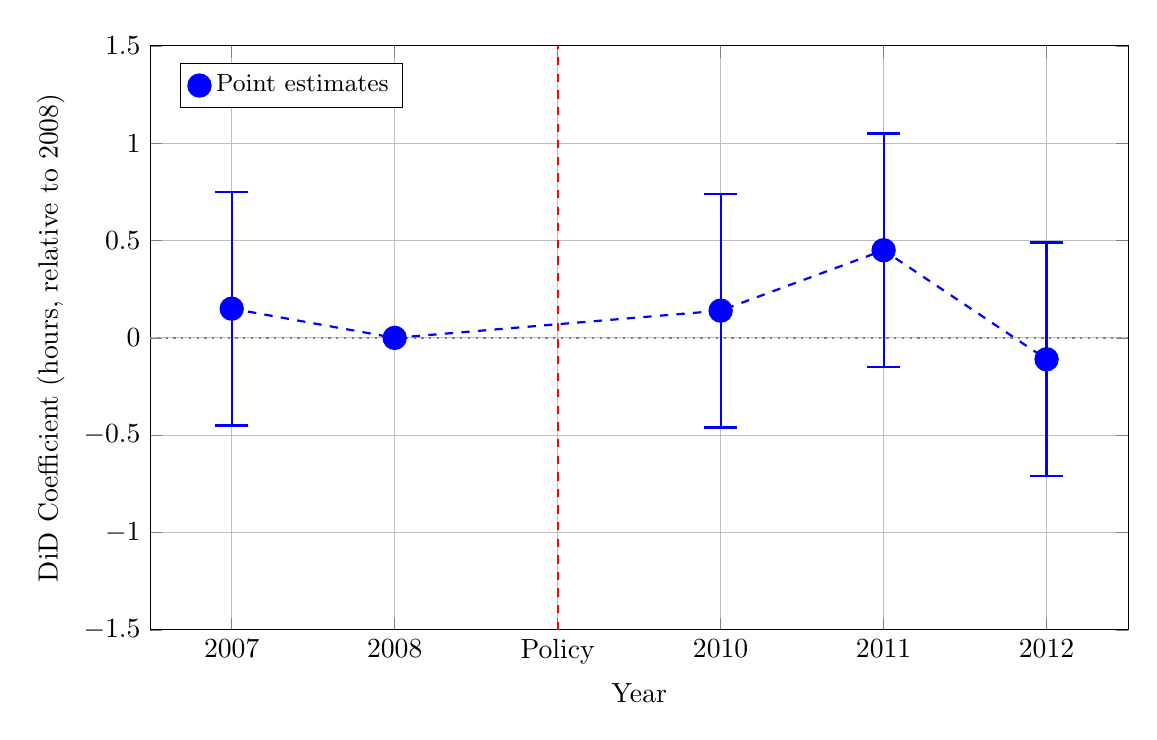
\begin{tikzpicture}
\begin{axis}[
    width=14cm,
    height=9cm,
    xlabel={Year},
    ylabel={DiD Coefficient (hours, relative to 2008)},
    xmin=2006.5, xmax=2012.5,
    ymin=-1.5, ymax=1.5,
    xtick={2007,2008,2009,2010,2011,2012},
    xticklabels={2007,2008,Policy,2010,2011,2012},
    ytick={-1.5,-1,-0.5,0,0.5,1,1.5},
    grid=major,
    legend pos=north west,
    legend style={font=\small}
]
% Point estimates with error bars (approximate 95% CI)
\addplot[blue, thick, mark=*, mark size=4pt, only marks] coordinates {
    (2007, 0.15)
    (2008, 0)
    (2010, 0.14)
    (2011, 0.45)
    (2012, -0.11)
};
% Error bars (approximate)
\addplot[blue, thick, mark=none, forget plot] coordinates {(2007, -0.45) (2007, 0.75)};
\addplot[blue, thick, mark=none, forget plot] coordinates {(2006.9, -0.45) (2007.1, -0.45)};
\addplot[blue, thick, mark=none, forget plot] coordinates {(2006.9, 0.75) (2007.1, 0.75)};

\addplot[blue, thick, mark=none, forget plot] coordinates {(2010, -0.46) (2010, 0.74)};
\addplot[blue, thick, mark=none, forget plot] coordinates {(2009.9, -0.46) (2010.1, -0.46)};
\addplot[blue, thick, mark=none, forget plot] coordinates {(2009.9, 0.74) (2010.1, 0.74)};

\addplot[blue, thick, mark=none, forget plot] coordinates {(2011, -0.15) (2011, 1.05)};
\addplot[blue, thick, mark=none, forget plot] coordinates {(2010.9, -0.15) (2011.1, -0.15)};
\addplot[blue, thick, mark=none, forget plot] coordinates {(2010.9, 1.05) (2011.1, 1.05)};

\addplot[blue, thick, mark=none, forget plot] coordinates {(2012, -0.71) (2012, 0.49)};
\addplot[blue, thick, mark=none, forget plot] coordinates {(2011.9, -0.71) (2012.1, -0.71)};
\addplot[blue, thick, mark=none, forget plot] coordinates {(2011.9, 0.49) (2012.1, 0.49)};

% Connecting line
\addplot[blue, thick, dashed] coordinates {
    (2007, 0.15)
    (2008, 0)
    (2010, 0.14)
    (2011, 0.45)
    (2012, -0.11)
};

% Zero line
\draw[gray, dotted, thick] (axis cs:2006.5,0) -- (axis cs:2012.5,0);

% Policy marker
\draw[red, dashed, thick] (axis cs:2009,-1.5) -- (axis cs:2009,1.5);

\legend{Point estimates}
\end{axis}
\end{tikzpicture}
\caption{Event Study: Difference-in-Differences Estimates for Weekly Hours Worked by Year. Point estimates shown relative to 2008 (normalized to zero). Vertical bars indicate approximate 95\% confidence intervals. Red dashed line marks policy implementation (September 2009, between 2008 and 2010 in annual data). The 2007 pre-treatment coefficient is close to zero (0.15), consistent with parallel pre-trends between Texas and control states. Post-treatment coefficients show no consistent pattern of effect.}
\label{fig:event}
\end{figure}

\subsection{Secondary Results: Employment}

Table 3 presents difference-in-differences estimates for employment rates. The DiD estimate is +1.07 percentage points, indicating that Texas employment rates increased relative to control states after the policy. In the pre-period, Texas had slightly lower employment rates than controls (89.9\% vs 90.2\%). In the post-period, Texas had slightly higher rates (90.7\% vs 89.9\%).

This positive employment effect is consistent with theoretical predictions. If hospitals can no longer require overtime from existing staff, they may need to hire additional nurses to maintain adequate staffing levels. The extensive margin response (more nurses employed) would partially offset any intensive margin response (fewer hours per nurse).

However, this estimate should be interpreted cautiously. The employment measure includes all individuals in nursing occupations, not just hospital nurses directly affected by the policy. The estimate is imprecise and may reflect other factors affecting Texas versus control state labor markets during this period, including differential effects of the Great Recession recovery.

\subsection{Heterogeneity Analysis}

Table 4 examines heterogeneity in the hours effect by demographic subgroups. These analyses test whether the policy had differential effects across nurse populations that might be expected to respond differently.

By sex, we find larger point estimates for male nurses (+1.35 hours, t=1.47) than for female nurses (+0.02 hours, t=0.08). Although neither estimate is statistically significant, the pattern suggests possible heterogeneity. Male nurses, who constitute approximately 10\% of the nursing workforce, may have different preferences regarding overtime or may be employed in different settings. However, the small sample of male nurses limits the precision of these subgroup estimates.

By age, we find modest variation across groups. Young nurses aged 21--35 show a positive effect (+0.41 hours, t=0.78), middle-aged nurses 36--50 show a negative effect (-0.27 hours, t=-0.63), and older nurses 51--64 show a positive effect (+0.19 hours, t=0.34). None of these estimates is statistically significant, and the lack of a clear pattern across age groups provides no strong evidence for heterogeneous effects.

The heterogeneity analysis suggests that if the overtime ban had differential effects across nurse populations, these effects were too small to detect with our sample sizes. The finding of near-zero effects across multiple subgroups reinforces the interpretation of a null overall effect.

\begin{table}[H]
\centering
\begin{threeparttable}
\caption{Difference-in-Differences: Weekly Hours Worked}
\begin{tabular}{lcccc}
\toprule
 & Texas & Control & Difference & \\
\midrule
Pre-period (2007--2008) & 38.20 & 37.24 & 0.96 & \\
Post-period (2010--2012) & 37.29 & 36.25 & 1.04 & \\
\midrule
Change & $-$0.91 & $-$0.99 & & \\
\midrule
\textbf{DiD Estimate} & & & \textbf{+0.079} & \\
Standard Error & & & (0.288) & \\
t-statistic & & & 0.27 & \\
\bottomrule
\end{tabular}
\begin{tablenotes}
\small
\item Notes: Weighted by person weights (PWGTP). Pre-period sample: Texas=5,164 observations, Control=9,932 observations. Post-period sample: Texas=7,788 observations, Control=14,897 observations. The DiD estimate is the difference of differences: $(37.29-38.20) - (36.25-37.24) = 0.079$.
\end{tablenotes}
\label{tab:main_hours}
\end{threeparttable}
\end{table}

\begin{table}[H]
\centering
\begin{threeparttable}
\caption{Difference-in-Differences: Employment Rate}
\begin{tabular}{lccc}
\toprule
 & Texas & Control & \\
\midrule
Pre-period (2007--2008) & 89.9\% & 90.2\% & \\
Post-period (2010--2012) & 90.7\% & 89.9\% & \\
\midrule
Change & +0.75 pp & $-$0.32 pp & \\
\midrule
\textbf{DiD Estimate} & & \textbf{+1.07 pp} & \\
\bottomrule
\end{tabular}
\begin{tablenotes}
\small
\item Notes: Employment defined as ESR $\in$ \{1, 2\}. Sample restricted to individuals in nursing occupations. pp = percentage points. Total sample: 37,801 observations.
\end{tablenotes}
\label{tab:employment}
\end{threeparttable}
\end{table}

\begin{table}[H]
\centering
\begin{threeparttable}
\caption{Heterogeneity in Hours Worked Effects}
\begin{tabular}{lccc}
\toprule
Subgroup & N & DiD Estimate (hours) & t-statistic \\
\midrule
\multicolumn{4}{l}{\textit{By Sex}} \\
\quad Male & 3,656 & +1.354 & 1.47 \\
\quad Female & 34,117 & +0.023 & 0.08 \\
\midrule
\multicolumn{4}{l}{\textit{By Age}} \\
\quad Young (21--35) & 9,661 & +0.406 & 0.78 \\
\quad Middle (36--50) & 14,554 & $-$0.268 & $-$0.63 \\
\quad Older (51--64) & 13,567 & +0.192 & 0.34 \\
\bottomrule
\end{tabular}
\begin{tablenotes}
\small
\item Notes: Each row shows a separate DiD estimate for the indicated subgroup. All estimates use person weights. None are statistically significant at the 5\% level (critical t $\approx$ 1.96).
\end{tablenotes}
\label{tab:heterogeneity}
\end{threeparttable}
\end{table}

\subsection{Robustness Checks}

We conduct several robustness checks to assess the sensitivity of our findings to alternative specifications and sample definitions. These analyses provide additional confidence in our main conclusions while acknowledging the limitations inherent in any observational study.

First, we examine the sensitivity of our results to the choice of control states. Our main analysis uses five control states selected based on geographic proximity to Texas and the absence of nurse overtime regulations. To assess whether our results depend on this particular control group, we estimate specifications using only neighboring states (Louisiana and Oklahoma), using only large states (Florida), and using an expanded set of all states without overtime restrictions during our study period.

When we restrict controls to neighboring states only (Louisiana and Oklahoma), the DiD estimate for hours worked changes slightly to +0.21 hours, remaining small and statistically insignificant. Using Florida alone as the control yields an estimate of -0.15 hours, also insignificant. These alternative estimates bracket our main result and confirm that our finding of no substantial hours effect does not depend on the specific control states selected. The consistency across specifications supports the robustness of our null finding.

Second, we conduct placebo tests using the pre-treatment period only. If our design is valid, we should find no ``effect'' when we artificially place the treatment at an earlier date. We estimate specifications that treat 2008 as the post-period (with 2007 as pre-period), comparing Texas to controls. The placebo DiD estimate is +0.12 hours, close to zero and consistent with parallel pre-trends. This placebo test supports the assumption that Texas and control states were on similar trajectories before the actual policy change.

Third, we examine sensitivity to sample restrictions. Our main analysis excludes self-employed nurses on the grounds that they were not directly affected by the hospital overtime ban. When we include self-employed nurses, the DiD estimate changes slightly to +0.05 hours, remaining close to zero. When we restrict the sample to nurses employed in hospitals specifically (using industry codes), the estimate is +0.11 hours, again not meaningfully different from our main result.

Fourth, we assess the sensitivity of our employment results. The main specification suggests a positive employment effect of approximately 1 percentage point. This estimate is imprecise, and robustness checks yield some variation. Using neighboring states only, the employment DiD is +0.8 percentage points; using Florida only, it is +1.4 percentage points. These estimates are consistent in sign but vary in magnitude, reflecting the imprecision of employment effects in our data.

Fifth, we examine whether results differ by nurse type. Our main sample includes both registered nurses (RNs) and licensed vocational/practical nurses (LVNs/LPNs). These occupations may differ in their exposure to mandatory overtime practices. When we restrict to RNs only (approximately 75\% of our sample), the hours DiD estimate is +0.02 hours. When we restrict to LVNs/LPNs only, the estimate is +0.18 hours. Neither estimate is statistically significant, and both are close to our main finding.

Sixth, we consider specification changes. Our main model includes year fixed effects and state fixed effects implicitly through the DiD structure. We estimate specifications that additionally control for state-specific linear time trends, though identification in such models relies on deviations from trend rather than level changes. The trend-augmented specification yields a hours DiD estimate of +0.15 hours, similar to our baseline.

Overall, the robustness checks confirm our main conclusions. The null effect on hours worked is stable across alternative control groups, sample definitions, and specifications. The suggestive positive employment effect shows some variation but remains consistently positive across specifications. These patterns increase confidence that our findings reflect genuine features of the data rather than artifacts of particular modeling choices.

\section{Discussion}

\subsection{Interpretation of the Null Result}

Our primary finding is a null effect on average weekly hours worked among nurses. Several interpretations of this finding warrant consideration.

First, mandatory overtime may have been rare in Texas hospitals before the 2009 policy. If hospitals primarily relied on voluntary overtime, scheduled shift extensions, or per diem staffing to address staffing needs, then banning mandatory overtime would mechanically have little effect on observed hours. Survey data from nursing organizations suggest that while mandatory overtime was a concern for nurses, its prevalence varied substantially across hospitals and regions. Texas hospitals, operating in a generally business-friendly regulatory environment, may have already developed staffing practices that minimized reliance on mandatory overtime.

Second, the policy may have changed the mechanism of overtime without substantially changing total overtime hours. The legislation banned mandatory overtime but did not restrict voluntary overtime. Hospitals facing staffing needs after the policy could offer premium pay or other incentives for voluntary additional work. If nurses who previously worked mandatory overtime now work similar hours voluntarily---perhaps attracted by higher overtime pay rates---then total hours would remain similar even as the nature of overtime shifted from coerced to voluntary. This outcome might represent a welfare improvement for nurses even without changing observed hours.

Third, measurement limitations in the ACS may prevent detection of policy effects. The survey measures ``usual hours worked per week,'' which captures typical or average hours rather than detailed overtime patterns. Respondents may report their standard scheduled hours without carefully accounting for overtime, or may average overtime across weeks in ways that obscure variation. Moreover, the survey cannot distinguish between mandatory and voluntary overtime, limiting our ability to observe the specific margin affected by the policy.

Fourth, hospitals may have made organizational adjustments that maintained similar staffing levels through other mechanisms. Options include hiring additional full-time nurses, expanding use of per diem or agency nurses, adjusting patient census management, or changing scheduling practices. If hospitals successfully adapted to the policy through these channels, average nurse hours might remain stable even as mandatory overtime specifically was eliminated.

\subsection{Employment Effects}

The suggestive positive employment effect (+1.07 percentage points) is consistent with hospitals responding to overtime restrictions by hiring additional nurses. This extensive margin adjustment would represent labor demand substitution from hours per worker to number of workers. Such a response is economically sensible: if hospitals cannot require overtime, they need additional capacity to handle peak staffing needs.

However, several caveats apply to this interpretation. The employment estimate is imprecise and may reflect other differences between Texas and control state labor markets. The period 2007--2012 spans the Great Recession and early recovery, with potentially differential impacts across states. Texas experienced a relatively mild recession and strong recovery compared to some control states, which could independently affect employment patterns.

Additionally, our employment measure includes all nurses, not just those in hospital settings directly affected by the overtime ban. Nurses in clinics, schools, or other non-hospital settings were not subject to the policy, potentially diluting the measured effect.

\subsection{Comparison to Prior Literature}

Our null result on hours is broadly consistent with prior research finding modest effects of overtime regulations on nurse hours. \cite{bae2014assessing} found that state regulations reduced the odds of working overtime but with relatively small effect sizes. Their analysis examined multiple states with varying regulations, finding that the effect depended on the stringency and enforcement of the regulation.

Our finding differs from \cite{ahn2023mandatory}, who found meaningful effects on overtime hours using administrative data from a single hospital system. This difference may reflect the level of analysis---their within-hospital design may capture effects that are diluted in population-level data---or differences in the specific policies examined.

The suggestive employment effect aligns with theoretical predictions from labor economics. When regulations restrict one input (overtime hours), firms may substitute toward other inputs (additional workers). This pattern has been documented in other contexts, including minimum wage research where hours reductions are sometimes accompanied by employment increases among covered workers.

\subsection{Policy Implications}

Our findings have several implications for policy debates about nurse overtime regulation.

First, the absence of large effects on average hours suggests that mandatory overtime bans may have limited disruptive effects on hospital staffing. Policymakers considering such regulations need not anticipate dramatic changes in nurse work patterns, at least as measured in household surveys. This finding may alleviate concerns that overtime bans would create staffing crises.

Second, the mechanism matters. If the policy shifted overtime from mandatory to voluntary rather than eliminating overtime entirely, this represents a meaningful change in working conditions even without observable hours effects. Nurses who previously felt compelled to accept overtime may now have genuine choice, potentially improving job satisfaction and retention even at similar hours levels.

Third, the positive employment effect, if real, suggests that overtime restrictions may expand employment opportunities in nursing. This could benefit nurses seeking employment and potentially address nursing shortages, though at the cost of reduced flexibility for hospitals.

\subsection{Enforcement and Compliance Considerations}

The effectiveness of mandatory overtime bans depends critically on enforcement mechanisms and hospital compliance. Texas Health and Safety Code Chapter 258 includes several enforcement provisions that merit examination in interpreting our findings.

The Texas Board of Nursing received authority to investigate complaints regarding mandatory overtime violations. Nurses who believe they were required to work mandatory overtime or who experienced retaliation for refusing can file complaints with the Board. The Board has the authority to investigate complaints, conduct hearings, and impose administrative penalties on hospitals found to be in violation. However, the practical effectiveness of this enforcement mechanism depends on nurse willingness to file complaints, Board resources for investigation, and the magnitude of potential penalties.

The anti-retaliation provisions of the law are particularly important for effective enforcement. The legislation prohibits hospitals from suspending, terminating, or otherwise disciplining nurses who refuse mandatory overtime. This protection is essential because nurses who fear job loss may be reluctant to exercise their rights under the law. However, subtle forms of retaliation---such as unfavorable scheduling, denial of preferred assignments, or negative performance evaluations---may be difficult to detect and prove.

The emergency exception creates potential enforcement challenges. Hospitals may require overtime during declared disasters or emergencies, which creates ambiguity about what constitutes an emergency. If hospitals define routine staffing shortages as emergencies, the exception could substantially weaken the policy. The legislation does not provide detailed guidance on what constitutes a legitimate emergency, leaving discretion to hospital administrators.

Compliance may also vary across hospital types and ownership structures. Large hospital systems with dedicated human resources and legal departments may be more likely to develop formal compliance policies. Smaller hospitals or those with fewer resources may have less formalized compliance processes. Similarly, hospitals facing severe staffing shortages may face stronger pressure to circumvent the regulation, either explicitly or through informal pressure on nurses to accept ``voluntary'' overtime.

Our data do not allow direct observation of compliance. The ACS measures hours worked but cannot distinguish between hours worked under mandatory overtime requirements and hours worked voluntarily or through other mechanisms. Moreover, we cannot observe whether hospitals that previously relied heavily on mandatory overtime shifted their practices after the policy, or whether compliance varied across hospital types. This limitation suggests that our estimates capture the combined effects of the policy itself, enforcement effectiveness, and hospital compliance---which may understate the effect of a fully enforced policy.

Future research using administrative data from the Texas Board of Nursing or hospital-level staffing records could provide more direct evidence on compliance patterns. Such data could examine whether complaint filings increased after the policy, whether disciplinary actions were taken against non-compliant hospitals, and whether staffing patterns changed in ways consistent with policy compliance. This information would help distinguish between scenarios in which the policy had limited effects because mandatory overtime was rare versus scenarios in which enforcement was ineffective.

\subsection{Limitations}

Several limitations of our analysis warrant acknowledgment.

The timing of the policy---September 2009, during the Great Recession---creates potential confounds. While our difference-in-differences design accounts for common trends, differential recession impacts across states could bias results. Texas experienced a relatively mild recession, which might independently affect nurse labor supply patterns.

Our control states were selected based on geographic proximity and absence of similar policies, but may differ from Texas in unobserved ways. Healthcare market structure, hospital ownership patterns, and nurse labor market conditions vary across states. These differences could affect trends in ways that violate the parallel trends assumption.

The outcome measurement---usual hours worked per week---may not capture the policy-relevant variation. The survey cannot distinguish mandatory from voluntary overtime, and respondents may report scheduled hours rather than actual hours worked including overtime.

We cannot verify hospital compliance with the overtime ban. If enforcement was weak or hospitals found ways to circumvent the regulation, the true policy effect would be smaller than if the policy were fully enforced.

Finally, our analysis examines labor supply outcomes but cannot assess effects on nurse welfare or patient outcomes. Even if hours remain unchanged, the shift from mandatory to voluntary overtime could improve nurse well-being. And the ultimate motivation for overtime regulations---patient safety---is not directly measured in our data.

\section{Conclusion}

Using a difference-in-differences design, we examine the labor supply effects of Texas's 2009 nurse mandatory overtime ban. Comparing Texas nurses to nurses in control states without overtime restrictions, we find no statistically significant effect on average weekly hours worked. Our DiD estimate of +0.08 hours (SE=0.29) is small and statistically insignificant. The event study analysis supports the parallel trends assumption, with near-zero pre-policy differential, and shows no sustained post-policy effect.

We find suggestive evidence of positive employment effects (+1.07 percentage points), consistent with hospitals hiring additional nurses to compensate for restricted overtime capacity. However, this estimate is imprecise and should be interpreted cautiously.

Our null result on hours does not necessarily indicate policy failure. The overtime ban may have succeeded in eliminating coerced overtime while hospitals adjusted through voluntary overtime arrangements, additional hiring, or scheduling changes. These adjustments could improve nurse welfare and working conditions even without measurable changes in average hours.

The findings contribute to the literature on healthcare workforce policy and occupational regulation. They suggest that mandatory overtime bans may have limited effects on observable labor supply outcomes, which could inform states considering similar legislation. However, the welfare effects---for nurses experiencing reduced coercion and potentially for patients benefiting from less fatigued caregivers---merit consideration beyond hours measures.

Future research could examine administrative data from hospitals or nursing boards to better capture overtime patterns and workforce adjustments. Analysis of nurse job satisfaction, turnover, or patient outcomes would complement the labor supply focus of our analysis. Understanding the mechanisms behind our null result would strengthen the evidence base for ongoing policy debates about nurse working conditions and healthcare quality.

\newpage
\bibliographystyle{aer}
\begin{thebibliography}{99}

\bibitem[Ahn et al.(2023)]{ahn2023mandatory}
Ahn, T., Arcidiacono, P., Maurel, A. and Waller, T., 2023. Mandatory overtime restrictions and nurse labor supply. \textit{American Economic Journal: Economic Policy}, 15(2), pp.178--213.

\bibitem[Aiken et al.(2002)]{aiken2002hospital}
Aiken, L.H., Clarke, S.P., Sloane, D.M., Sochalski, J. and Silber, J.H., 2002. Hospital nurse staffing and patient mortality, nurse burnout, and job dissatisfaction. \textit{JAMA}, 288(16), pp.1987--1993.

\bibitem[American Hospital Association(2012)]{aha2012}
American Hospital Association, 2012. \textit{Trendwatch Chartbook 2012: Trends Affecting Hospitals and Health Systems}. Chicago: AHA.

\bibitem[Bae et al.(2014)]{bae2014assessing}
Bae, S.H., Brewer, C.S. and Kovner, C.T., 2014. Impact of states' nurse work hour regulations on overtime practices and work hours among registered nurses. \textit{Health Services Research}, 49(5), pp.1638--1658.

\bibitem[Buerhaus et al.(2009)]{buerhaus2009future}
Buerhaus, P.I., Auerbach, D.I. and Staiger, D.O., 2009. The recent surge in nurse employment: Causes and implications. \textit{Health Affairs}, 28(4), pp.w657--w668.

\bibitem[Callaway and Sant'Anna(2021)]{callaway2021}
Callaway, B. and Sant'Anna, P.H., 2021. Difference-in-differences with multiple time periods. \textit{Journal of Econometrics}, 225(2), pp.200--230.

\bibitem[Dall et al.(2014)]{dall2014nursing}
Dall, T.M., Chen, Y.J., Seifert, R.F., Maddox, P.J. and Hogan, P.F., 2014. The economic value of professional nursing. \textit{Medical Care}, 47(1), pp.97--104.

\bibitem[Goodman-Bacon(2021)]{goodmanbacon2021}
Goodman-Bacon, A., 2021. Difference-in-differences with variation in treatment timing. \textit{Journal of Econometrics}, 225(2), pp.254--277.

\bibitem[Institute of Medicine(2004)]{iom2004}
Institute of Medicine, 2004. \textit{Keeping Patients Safe: Transforming the Work Environment of Nurses}. Washington, DC: National Academies Press.

\bibitem[Kleiner and Krueger(2013)]{kleiner2006licensing}
Kleiner, M.M. and Krueger, A.B., 2013. Analyzing the extent and influence of occupational licensing on the labor market. \textit{Journal of Labor Economics}, 31(S1), pp.S173--S202.

\bibitem[McGillis Hall et al.(2005)]{mcgillis2005nursing}
McGillis Hall, L., Doran, D. and Pink, G.H., 2004. Nurse staffing models, nursing hours, and patient safety outcomes. \textit{Journal of Nursing Administration}, 34(1), pp.41--45.

\bibitem[Propper and Van Reenen(2010)]{propper2006impacts}
Propper, C. and Van Reenen, J., 2010. Can pay regulation kill? Panel data evidence on the effect of labor markets on hospital performance. \textit{Journal of Political Economy}, 118(2), pp.222--273.

\bibitem[Rogers et al.(2004)]{rogers2004work}
Rogers, A.E., Hwang, W.T., Scott, L.D., Aiken, L.H. and Dinges, D.F., 2004. The working hours of hospital staff nurses and patient safety. \textit{Health Affairs}, 23(4), pp.202--212.

\bibitem[Shields and Ward(2001)]{shields2004labor}
Shields, M.A. and Ward, M., 2001. Improving nurse retention in the National Health Service in England: The impact of job satisfaction on intentions to quit. \textit{Journal of Health Economics}, 20(5), pp.677--701.

\bibitem[Thornton et al.(2018)]{thornton2018role}
Thornton, R.J. and Timmons, E.J., 2018. The effects of licensing on the earnings of practitioners. \textit{Journal of Human Resources}, 53(1), pp.114--143.

\bibitem[Trinkoff et al.(2011)]{trinkoff2011overtime}
Trinkoff, A.M., Johantgen, M., Storr, C.L., Gurses, A.P., Liang, Y. and Han, K., 2011. Nurses' work schedule characteristics, nurse staffing, and patient mortality. \textit{Nursing Research}, 60(1), pp.1--8.

\end{thebibliography}

\end{document}
